% Klassenarbeit Mathe 9b 2.3.2017

\documentclass[a4paper,ngerman,12pt]{exam}
\usepackage[a4paper, total={16cm, 26cm}]{geometry}
\usepackage[utf8]{inputenc}
\usepackage{amsfonts}
\usepackage{amsmath}
\usepackage{ngerman}
%\usepackage{gensymb}
\usepackage{tabularx}
\usepackage{url}
\usepackage{tikz}
\usepackage{tkz-euclide}
\usepackage{rotating}
%\usetkzobj{all}
\usetikzlibrary{calc}
\usepackage{pgfplots}
\pgfplotsset{
  compat=1.12,
  axis lines=middle
}


\makeatletter
\def\rechterWinkel{\@ifnextchar[\rechterWinkel@i\rechterWinkel@ii}
\def\rechterWinkel@i[#1](#2,#3,#4){%
  \pgfmathsetmacro{\pos@A}{0.5*#1}
  \pgfmathsetmacro{\pos@B}{0.25*#1}
   \tkzMarkAngle[size=\pos@A](#2,#3,#4)
   \tkzLabelAngle[pos=\pos@B](#2,#3,#4){\tikz \fill (0,0) circle (0.6pt);}
}% 
\def\rechterWinkel@ii(#1,#2,#3){%  
\rechterWinkel@i[1](#1,#2,#3)
}% 
\makeatother

\pointpoints{Punkt}{Punkte}
\bonuspointpoints{Bonuspunkt}{Bonuspunkte}
\renewcommand{\solutiontitle}{\noindent\textbf{Lösung:}%
\enspace}

\runningfooter{Klasse 9b}{Klassenarbeit Mathematik, 2.3.2017}{Seite \thepage\ von \numpages}
\runningfootrule

\chqword{Frage}
\chpgword{Seite}
\chpword{Punkte}
\chbpword{Bonus Punkte}
\chsword{Erreicht}
\chtword{Gesamt}

\hpword{Punkte:} % Punktetabelle
\hsword{Ergebnis:}
\hqword{Aufgabe:}
\htword{Summe}

\begin{document}
\noindent {\bf Name}:\\
\noindent {\bf Vorname}:\\
\hrule

\begin{center}
{\large\bf Klassenarbeit zur Ähnlichkeit}\\[2mm]
 mit Aufgaben zum Höhensatz des Euklid und zu Linearen Funktionen\\
Hilfsmittel: Geodreick, Zirkel und Taschenrechner
\end{center}
Gymnasium Tiergarten\hfill 2. März 2017\\
Klasse 9b, Mathematik\hfill Bearbeitungszeit: 60 Minuten

\begin{center}
\addpoints\gradetable[h][questions] 
\end{center}
\hrule
\medskip

%%%%%%%%%%%%%%%%%%%%%%%%%%%%%%%%%%%%
\begin{questions}

\question \underline{Höhensatz des Euklid}: Schaue Dir den folgenden Querschnitt durch einen Tunnel an. Die Straße ist zweispurig mit Gegenverkehr (es müssen also zwei Autos aneinander vorbei fahren können). Links und rechts gibt es jeweils einen Gehsteig. Das Deckengewölbe entspricht einem Halbkreis mit Mittelpunkt genau auf dem Mittelstreifen. Normalerweise gibt es am Eingang des Tunnels ein Schild, das die Durchfahrtshöhe angibt. Leider ist das Schild verschwunden.\par
\begin{center}\includegraphics[width=.6\textwidth]{tunnel.png}\end{center}
\par

\begin{parts}
\part[4] Berechne mit Hilfe des Höhensatzes des Euklid, wie hoch ein Auto maximal sein darf, um auf einem der Fahrstreifen durch den Tunnel zu passen.
\vfill
\part[2] Welche Zahl würdest Du auf das Schild schreiben? Begründe Deine Aussage.
\end{parts}
\pagebreak

\question Lineare Funktionen\par%\\[0.3cm]
\begin{center}
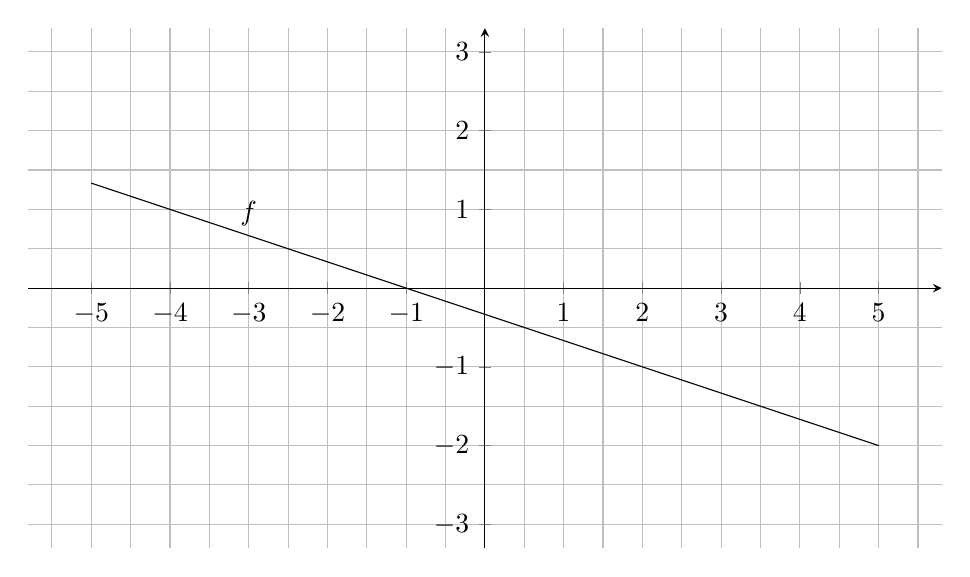
\begin{tikzpicture}
  \begin{axis}[
    xmin=-5.8,xmax=5.8,
    ymin=-3.3,ymax=3.3,
    x=1cm,
    y=1cm,
    minor tick num=1,% zwischen zwei Haupt-Achsmarkierungen jeweils einen Untermarkierungen einf?gen
    minor tick length=0pt,% L·nge der Untermarkierungen auf 0 setzen, sie also unterdr?cken
    grid={both}% Gitterlinien sowohl durch die Positionen der Haupt- als auch Untermarkierungen
    ]
    \addplot[color=black] {-(x+1)/3} node[above,pos=0.2] {$f$};
  \end{axis}
\end{tikzpicture}
\end{center}

\begin{parts}
\part[1] Miss die Werte von $f$ an den Stellen $x=-4$ und $x=2$.\\[1cm]
\part[2] Bestimme anhand der Messwerte die Steigung von $f$.\\[2cm]
\part[1] Zeichne eine zu $f$ parallele lineare Funktion $g$ mit Ordinatenabschnitt 1 in das obige Koordinatensystem ein.
\part[2] Stelle eine Funktionsgleichung für $g$ auf.\\[2cm]
\part[2] Berechne die Nullstelle von $g$, indem Du $y=0$ in die Funktionsgleichung einsetzt.\\[2cm]
\part[1] Gib die Funktionsgleichung einer zu $f$ und $g$ orthogonalen linearen Funktion an.
\end{parts}

\pagebreak

\question \underline{Ähnlichkeit}
\begin{parts}
\part[3] Definiere den Begriff Ähnlichkeit.\\[5cm]

\part[5] Welche der Dreiecke sind ähnlich zueinander, welche sind kongruent? Begründe Deine Aussagen.
\par\bigskip
\begin{center}
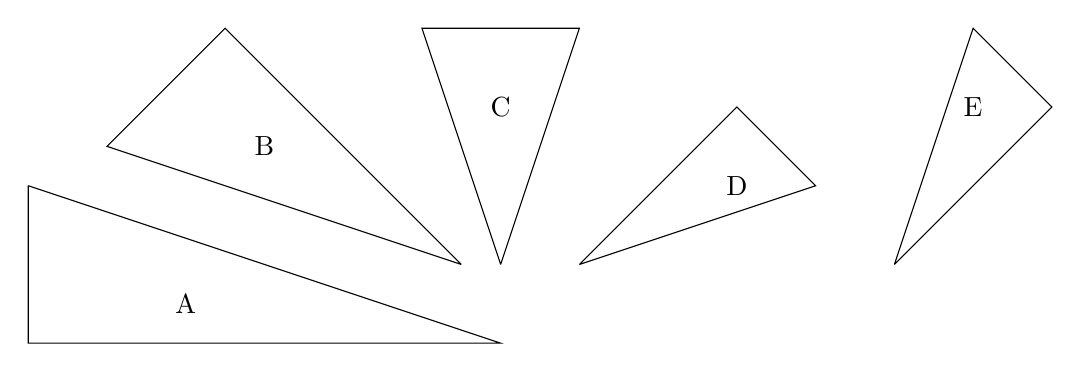
\begin{tikzpicture}[scale=1]
\tkzDefPoint(0,0){A}
\tkzDefPoint(3,1){B}  
\tkzDefPoint(2,2){C}  
\draw (A) -- (B) -- (C) -- (A);
\draw[color=black] (2,1) node {D};

\tkzDefPoint(4,0){A}
\tkzDefPoint(5,3){B}  
\tkzDefPoint(6,2){C} 
\draw (A) -- (B) -- (C) -- (A);
\draw[color=black] (5,2) node {E};

\tkzDefPoint(-1.5,0){A}
\tkzDefPoint(-6,1.5){B}  
\tkzDefPoint(-4.5,3){C}  
\draw (A) -- (B) -- (C) -- (A);
\draw[color=black] (-4,1.5) node {B};

\tkzDefPoint(-1,0){A}
\tkzDefPoint(-2,3){B}  
\tkzDefPoint(0,3){C} 
\draw (A) -- (B) -- (C) -- (A);
\draw[color=black] (-1,2) node {C};

\tkzDefPoint(-7,1){A}
\tkzDefPoint(-7,-1){B}  
\tkzDefPoint(-1,-1){C} 
\draw (A) -- (B) -- (C) -- (A);
\draw[color=black] (-5,-0.5) node {A};
\end{tikzpicture}
\end{center}
\vspace{5cm}

\part[2] Der Berliner Fernsehturm hat eine Höhe von 365 Metern. In welchem Maßstab ist er hier abgebildet?\\[-0.5cm]
\includegraphics[angle=90, width=0.7\textwidth]{Fernsehturm.png}
\end{parts}
\vfill
{\scriptsize Bildnachweis:\\
\url{https://de.wikipedia.org/wiki/Berliner_Fernsehturm#/media/File:Kontur-BerlinerFernsehturm.svg}\\
\url{http://www.lohnt-nicht.de/schule/Gym-Aichach/Mathe-9a/Lernpfad-Pythagoras/Inhalt/Hoehensatz.xhtml}}

\pagebreak

\question \underline{Zentrische Streckung}
\begin{flushright}
\begin{tikzpicture}[scale=1]
\tkzDefPoint(-1,0){A}
\tkzDefPoint(0,0){B}  
\tkzDefPoint(-1,-1){C}  
\tkzDefPoint(1.5,-0.5){D}  
\draw (A) -- (B) -- (C) -- (A);
\tkzDrawPoints(D);
\draw[color=black] (1.3,-0.7) node {$Z$};

\tkzDefPoint(4,-2){A}
\tkzDefPoint(7,-2){B}  
\tkzDefPoint(7,1){C}  
\tkzDefPoint(4,1){D} 
\draw (A) -- (B) -- (C) -- (D) -- (A);

\draw[color=white] (10,1) -- (10,0);
\end{tikzpicture}
\end{flushright}

\begin{parts}
\part[3] Strecke das Dreieck um den Streckfaktor 2 vom Streckzentrum $Z$.
\part[3] Strecke das Quadrat um den Streckfaktor $\frac{2}{3}$ vom Streckzentrum $Z$.
\part[1] Miss die Seitenlänge des Ursprungsquadrats und berechne den Flächeninhalt.\\[1cm]
\part[1] Berechne daraus mit Hilfe des Streckfaktors den Flächeninhalt des gestreckten Quadrats.\\[1cm]
\end{parts}
\par\medskip

\question Die folgende Figur hat insgesamt 9 Schnitt- bzw. Eckpunkte.
\begin{center}
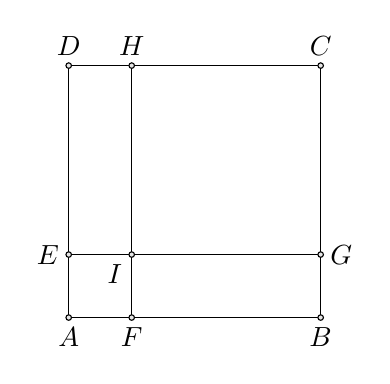
\begin{tikzpicture}[scale=0.8]
\tkzDefPoint(0,0){A}
\tkzDefPoint(0,4){B}  
\tkzDefPoint(4,4){C}  
\tkzDefPoint(4,0){D}
\tkzDefPoint(0,1){E}
\tkzDefPoint(1,0){F}
\tkzDefPoint(4,1){G}
\tkzDefPoint(1,4){H}
\tkzDefPoint(1,1){I}
\draw (A) node[below] {$A$} -- 
(B) node[above] {$D$} -- 
(C) node[above] {$C$} -- 
(D) node[below] {$B$} -- (A);
\draw (E) node[left] {$E$} -- (G) node[right] {$G$};
\draw (F) node[below] {$F$} -- (I) node[below left] {$I$} -- (H) node[above] {$H$};
\tkzDrawPoints(A, B, C, D, E, F, G, H, I);
\end{tikzpicture}
\end{center}
\begin{parts}
\part[3] Bestimme alle in der Figur enthaltenen Rechtecke und gib Ihre Eckpunkte an, z.B. $ABCD$ für das große Quadrat.\\[1.5cm]
\part[4] Welche der in der Figur enthaltenen Rechtecke sind ähnlich zueinander? Welche sind kongruent? Begründe Deine Aussagen.
\end{parts}
\end{questions}
\end{document}
